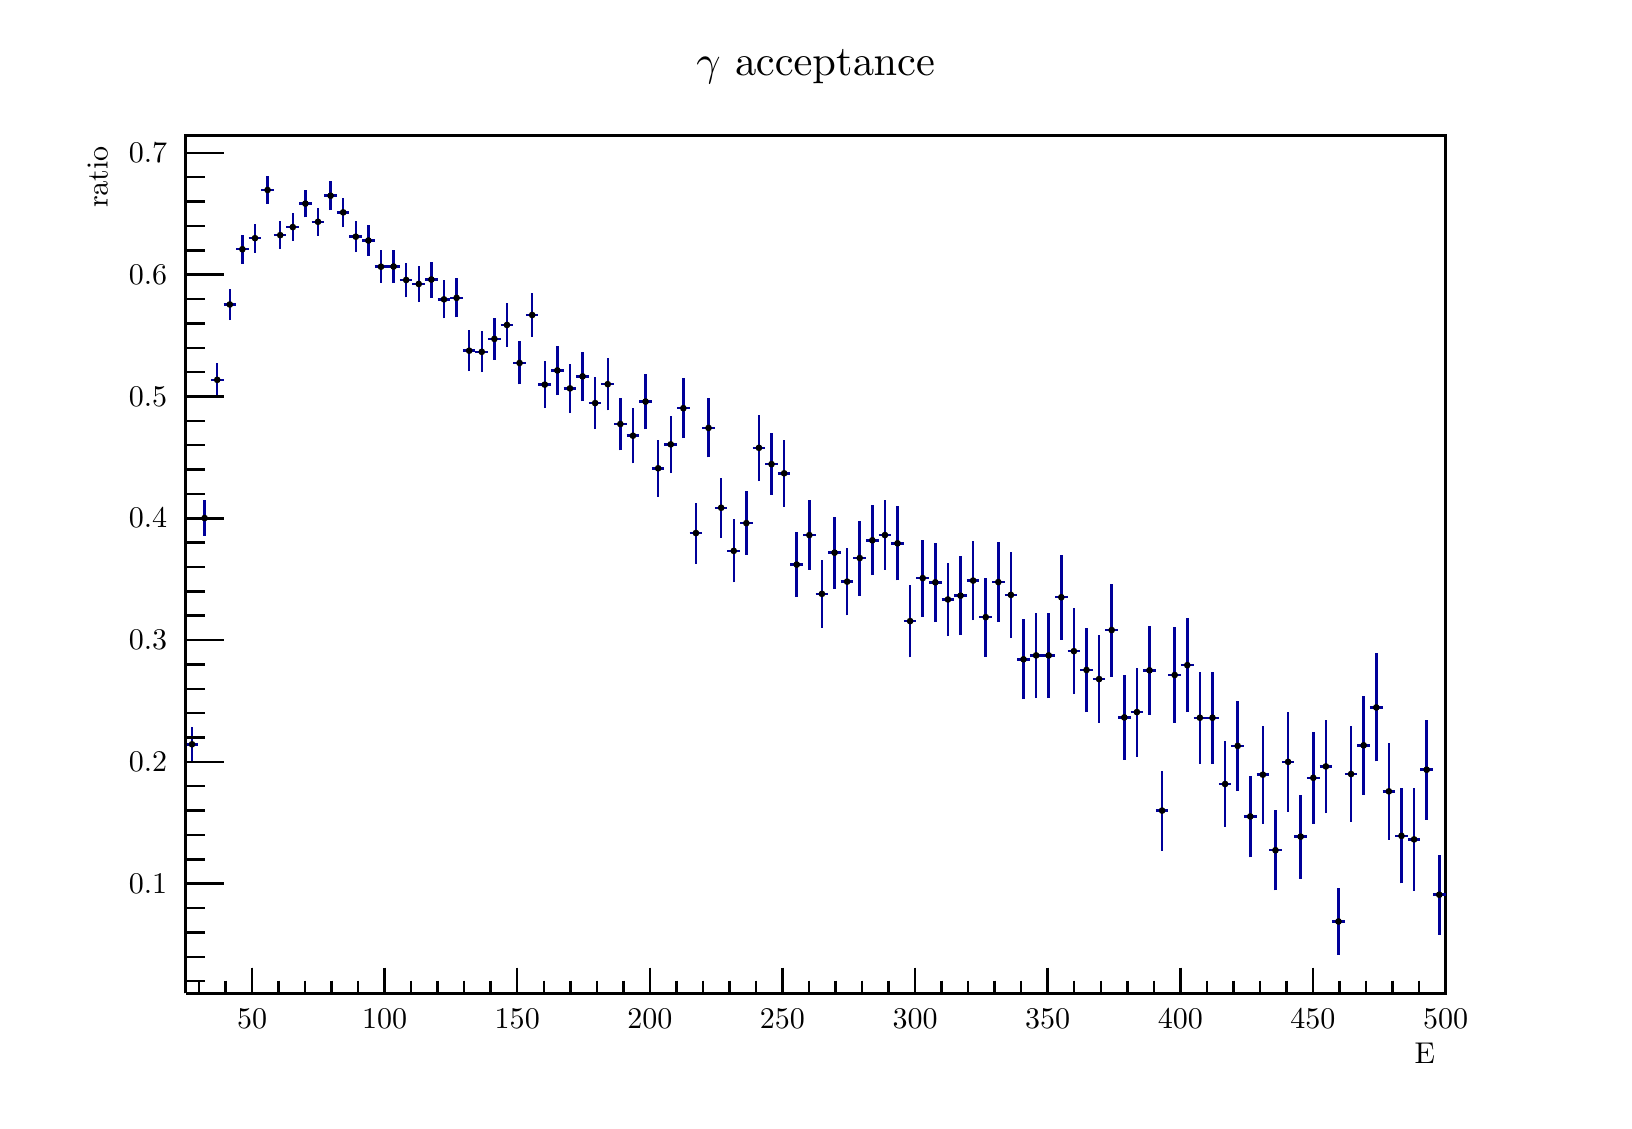
\begin{tikzpicture}
\pgfdeclareplotmark{cross} {
\pgfpathmoveto{\pgfpoint{-0.3\pgfplotmarksize}{\pgfplotmarksize}}
\pgfpathlineto{\pgfpoint{+0.3\pgfplotmarksize}{\pgfplotmarksize}}
\pgfpathlineto{\pgfpoint{+0.3\pgfplotmarksize}{0.3\pgfplotmarksize}}
\pgfpathlineto{\pgfpoint{+1\pgfplotmarksize}{0.3\pgfplotmarksize}}
\pgfpathlineto{\pgfpoint{+1\pgfplotmarksize}{-0.3\pgfplotmarksize}}
\pgfpathlineto{\pgfpoint{+0.3\pgfplotmarksize}{-0.3\pgfplotmarksize}}
\pgfpathlineto{\pgfpoint{+0.3\pgfplotmarksize}{-1.\pgfplotmarksize}}
\pgfpathlineto{\pgfpoint{-0.3\pgfplotmarksize}{-1.\pgfplotmarksize}}
\pgfpathlineto{\pgfpoint{-0.3\pgfplotmarksize}{-0.3\pgfplotmarksize}}
\pgfpathlineto{\pgfpoint{-1.\pgfplotmarksize}{-0.3\pgfplotmarksize}}
\pgfpathlineto{\pgfpoint{-1.\pgfplotmarksize}{0.3\pgfplotmarksize}}
\pgfpathlineto{\pgfpoint{-0.3\pgfplotmarksize}{0.3\pgfplotmarksize}}
\pgfpathclose
\pgfusepathqstroke
}
\pgfdeclareplotmark{cross*} {
\pgfpathmoveto{\pgfpoint{-0.3\pgfplotmarksize}{\pgfplotmarksize}}
\pgfpathlineto{\pgfpoint{+0.3\pgfplotmarksize}{\pgfplotmarksize}}
\pgfpathlineto{\pgfpoint{+0.3\pgfplotmarksize}{0.3\pgfplotmarksize}}
\pgfpathlineto{\pgfpoint{+1\pgfplotmarksize}{0.3\pgfplotmarksize}}
\pgfpathlineto{\pgfpoint{+1\pgfplotmarksize}{-0.3\pgfplotmarksize}}
\pgfpathlineto{\pgfpoint{+0.3\pgfplotmarksize}{-0.3\pgfplotmarksize}}
\pgfpathlineto{\pgfpoint{+0.3\pgfplotmarksize}{-1.\pgfplotmarksize}}
\pgfpathlineto{\pgfpoint{-0.3\pgfplotmarksize}{-1.\pgfplotmarksize}}
\pgfpathlineto{\pgfpoint{-0.3\pgfplotmarksize}{-0.3\pgfplotmarksize}}
\pgfpathlineto{\pgfpoint{-1.\pgfplotmarksize}{-0.3\pgfplotmarksize}}
\pgfpathlineto{\pgfpoint{-1.\pgfplotmarksize}{0.3\pgfplotmarksize}}
\pgfpathlineto{\pgfpoint{-0.3\pgfplotmarksize}{0.3\pgfplotmarksize}}
\pgfpathclose
\pgfusepathqfillstroke
}
\pgfdeclareplotmark{newstar} {
\pgfpathmoveto{\pgfqpoint{0pt}{\pgfplotmarksize}}
\pgfpathlineto{\pgfqpointpolar{44}{0.5\pgfplotmarksize}}
\pgfpathlineto{\pgfqpointpolar{18}{\pgfplotmarksize}}
\pgfpathlineto{\pgfqpointpolar{-20}{0.5\pgfplotmarksize}}
\pgfpathlineto{\pgfqpointpolar{-54}{\pgfplotmarksize}}
\pgfpathlineto{\pgfqpointpolar{-90}{0.5\pgfplotmarksize}}
\pgfpathlineto{\pgfqpointpolar{234}{\pgfplotmarksize}}
\pgfpathlineto{\pgfqpointpolar{198}{0.5\pgfplotmarksize}}
\pgfpathlineto{\pgfqpointpolar{162}{\pgfplotmarksize}}
\pgfpathlineto{\pgfqpointpolar{134}{0.5\pgfplotmarksize}}
\pgfpathclose
\pgfusepathqstroke
}
\pgfdeclareplotmark{newstar*} {
\pgfpathmoveto{\pgfqpoint{0pt}{\pgfplotmarksize}}
\pgfpathlineto{\pgfqpointpolar{44}{0.5\pgfplotmarksize}}
\pgfpathlineto{\pgfqpointpolar{18}{\pgfplotmarksize}}
\pgfpathlineto{\pgfqpointpolar{-20}{0.5\pgfplotmarksize}}
\pgfpathlineto{\pgfqpointpolar{-54}{\pgfplotmarksize}}
\pgfpathlineto{\pgfqpointpolar{-90}{0.5\pgfplotmarksize}}
\pgfpathlineto{\pgfqpointpolar{234}{\pgfplotmarksize}}
\pgfpathlineto{\pgfqpointpolar{198}{0.5\pgfplotmarksize}}
\pgfpathlineto{\pgfqpointpolar{162}{\pgfplotmarksize}}
\pgfpathlineto{\pgfqpointpolar{134}{0.5\pgfplotmarksize}}
\pgfpathclose
\pgfusepathqfillstroke
}
\definecolor{c}{rgb}{1,1,1};
\draw [color=c, fill=c] (0,0) rectangle (20,13.6207);
\draw [color=c, fill=c] (2,1.36207) rectangle (18,12.2586);
\definecolor{c}{rgb}{0,0,0};
\draw [c,line width=0.9] (2,1.36207) -- (2,12.2586) -- (18,12.2586) -- (18,1.36207) -- (2,1.36207);
\definecolor{c}{rgb}{1,1,1};
\draw [color=c, fill=c] (2,1.36207) rectangle (18,12.2586);
\definecolor{c}{rgb}{0,0,0};
\draw [c,line width=0.9] (2,1.36207) -- (2,12.2586) -- (18,12.2586) -- (18,1.36207) -- (2,1.36207);
\definecolor{c}{rgb}{0,0,0.6};
\draw [c,line width=0.9] (2.08,4.31355) -- (2.08,4.52684);
\draw [c,line width=0.9] (2.08,4.52684) -- (2.08,4.74014);
\draw [c,line width=0.9] (2,4.52684) -- (2.08,4.52684);
\draw [c,line width=0.9] (2.08,4.52684) -- (2.16,4.52684);
\definecolor{c}{rgb}{0,0,0};
\foreach \P in {(2.08,4.52684)}{\draw[mark options={color=c,fill=c},mark size=2.402402pt,mark=*,mark size=1pt] plot coordinates {\P};}
\definecolor{c}{rgb}{0,0,0.6};
\draw [c,line width=0.9] (2.24,7.17406) -- (2.24,7.39981);
\draw [c,line width=0.9] (2.24,7.39981) -- (2.24,7.62555);
\draw [c,line width=0.9] (2.16,7.39981) -- (2.24,7.39981);
\draw [c,line width=0.9] (2.24,7.39981) -- (2.32,7.39981);
\definecolor{c}{rgb}{0,0,0};
\foreach \P in {(2.24,7.39981)}{\draw[mark options={color=c,fill=c},mark size=2.402402pt,mark=*,mark size=1pt] plot coordinates {\P};}
\definecolor{c}{rgb}{0,0,0.6};
\draw [c,line width=0.9] (2.4,8.94204) -- (2.4,9.15484);
\draw [c,line width=0.9] (2.4,9.15484) -- (2.4,9.36764);
\draw [c,line width=0.9] (2.32,9.15484) -- (2.4,9.15484);
\draw [c,line width=0.9] (2.4,9.15484) -- (2.48,9.15484);
\definecolor{c}{rgb}{0,0,0};
\foreach \P in {(2.4,9.15484)}{\draw[mark options={color=c,fill=c},mark size=2.402402pt,mark=*,mark size=1pt] plot coordinates {\P};}
\definecolor{c}{rgb}{0,0,0.6};
\draw [c,line width=0.9] (2.56,9.91497) -- (2.56,10.1117);
\draw [c,line width=0.9] (2.56,10.1117) -- (2.56,10.3085);
\draw [c,line width=0.9] (2.48,10.1117) -- (2.56,10.1117);
\draw [c,line width=0.9] (2.56,10.1117) -- (2.64,10.1117);
\definecolor{c}{rgb}{0,0,0};
\foreach \P in {(2.56,10.1117)}{\draw[mark options={color=c,fill=c},mark size=2.402402pt,mark=*,mark size=1pt] plot coordinates {\P};}
\definecolor{c}{rgb}{0,0,0.6};
\draw [c,line width=0.9] (2.72,10.6291) -- (2.72,10.814);
\draw [c,line width=0.9] (2.72,10.814) -- (2.72,10.999);
\draw [c,line width=0.9] (2.64,10.814) -- (2.72,10.814);
\draw [c,line width=0.9] (2.72,10.814) -- (2.8,10.814);
\definecolor{c}{rgb}{0,0,0};
\foreach \P in {(2.72,10.814)}{\draw[mark options={color=c,fill=c},mark size=2.402402pt,mark=*,mark size=1pt] plot coordinates {\P};}
\definecolor{c}{rgb}{0,0,0.6};
\draw [c,line width=0.9] (2.88,10.771) -- (2.88,10.9546);
\draw [c,line width=0.9] (2.88,10.9546) -- (2.88,11.1383);
\draw [c,line width=0.9] (2.8,10.9546) -- (2.88,10.9546);
\draw [c,line width=0.9] (2.88,10.9546) -- (2.96,10.9546);
\definecolor{c}{rgb}{0,0,0};
\foreach \P in {(2.88,10.9546)}{\draw[mark options={color=c,fill=c},mark size=2.402402pt,mark=*,mark size=1pt] plot coordinates {\P};}
\definecolor{c}{rgb}{0,0,0.6};
\draw [c,line width=0.9] (3.04,11.3924) -- (3.04,11.5661);
\draw [c,line width=0.9] (3.04,11.5661) -- (3.04,11.7397);
\draw [c,line width=0.9] (2.96,11.5661) -- (3.04,11.5661);
\draw [c,line width=0.9] (3.04,11.5661) -- (3.12,11.5661);
\definecolor{c}{rgb}{0,0,0};
\foreach \P in {(3.04,11.5661)}{\draw[mark options={color=c,fill=c},mark size=2.402402pt,mark=*,mark size=1pt] plot coordinates {\P};}
\definecolor{c}{rgb}{0,0,0.6};
\draw [c,line width=0.9] (3.2,10.8142) -- (3.2,10.9928);
\draw [c,line width=0.9] (3.2,10.9928) -- (3.2,11.1714);
\draw [c,line width=0.9] (3.12,10.9928) -- (3.2,10.9928);
\draw [c,line width=0.9] (3.2,10.9928) -- (3.28,10.9928);
\definecolor{c}{rgb}{0,0,0};
\foreach \P in {(3.2,10.9928)}{\draw[mark options={color=c,fill=c},mark size=2.402402pt,mark=*,mark size=1pt] plot coordinates {\P};}
\definecolor{c}{rgb}{0,0,0.6};
\draw [c,line width=0.9] (3.36,10.9189) -- (3.36,11.0952);
\draw [c,line width=0.9] (3.36,11.0952) -- (3.36,11.2715);
\draw [c,line width=0.9] (3.28,11.0952) -- (3.36,11.0952);
\draw [c,line width=0.9] (3.36,11.0952) -- (3.44,11.0952);
\definecolor{c}{rgb}{0,0,0};
\foreach \P in {(3.36,11.0952)}{\draw[mark options={color=c,fill=c},mark size=2.402402pt,mark=*,mark size=1pt] plot coordinates {\P};}
\definecolor{c}{rgb}{0,0,0.6};
\draw [c,line width=0.9] (3.52,11.2185) -- (3.52,11.3932);
\draw [c,line width=0.9] (3.52,11.3932) -- (3.52,11.568);
\draw [c,line width=0.9] (3.44,11.3932) -- (3.52,11.3932);
\draw [c,line width=0.9] (3.52,11.3932) -- (3.6,11.3932);
\definecolor{c}{rgb}{0,0,0};
\foreach \P in {(3.52,11.3932)}{\draw[mark options={color=c,fill=c},mark size=2.402402pt,mark=*,mark size=1pt] plot coordinates {\P};}
\definecolor{c}{rgb}{0,0,0.6};
\draw [c,line width=0.9] (3.68,10.982) -- (3.68,11.1622);
\draw [c,line width=0.9] (3.68,11.1622) -- (3.68,11.3424);
\draw [c,line width=0.9] (3.6,11.1622) -- (3.68,11.1622);
\draw [c,line width=0.9] (3.68,11.1622) -- (3.76,11.1622);
\definecolor{c}{rgb}{0,0,0};
\foreach \P in {(3.68,11.1622)}{\draw[mark options={color=c,fill=c},mark size=2.402402pt,mark=*,mark size=1pt] plot coordinates {\P};}
\definecolor{c}{rgb}{0,0,0.6};
\draw [c,line width=0.9] (3.84,11.3112) -- (3.84,11.4932);
\draw [c,line width=0.9] (3.84,11.4932) -- (3.84,11.6751);
\draw [c,line width=0.9] (3.76,11.4932) -- (3.84,11.4932);
\draw [c,line width=0.9] (3.84,11.4932) -- (3.92,11.4932);
\definecolor{c}{rgb}{0,0,0};
\foreach \P in {(3.84,11.4932)}{\draw[mark options={color=c,fill=c},mark size=2.402402pt,mark=*,mark size=1pt] plot coordinates {\P};}
\definecolor{c}{rgb}{0,0,0.6};
\draw [c,line width=0.9] (4,11.0948) -- (4,11.2822);
\draw [c,line width=0.9] (4,11.2822) -- (4,11.4695);
\draw [c,line width=0.9] (3.92,11.2822) -- (4,11.2822);
\draw [c,line width=0.9] (4,11.2822) -- (4.08,11.2822);
\definecolor{c}{rgb}{0,0,0};
\foreach \P in {(4,11.2822)}{\draw[mark options={color=c,fill=c},mark size=2.402402pt,mark=*,mark size=1pt] plot coordinates {\P};}
\definecolor{c}{rgb}{0,0,0.6};
\draw [c,line width=0.9] (4.16,10.7761) -- (4.16,10.973);
\draw [c,line width=0.9] (4.16,10.973) -- (4.16,11.1699);
\draw [c,line width=0.9] (4.08,10.973) -- (4.16,10.973);
\draw [c,line width=0.9] (4.16,10.973) -- (4.24,10.973);
\definecolor{c}{rgb}{0,0,0};
\foreach \P in {(4.16,10.973)}{\draw[mark options={color=c,fill=c},mark size=2.402402pt,mark=*,mark size=1pt] plot coordinates {\P};}
\definecolor{c}{rgb}{0,0,0.6};
\draw [c,line width=0.9] (4.32,10.73) -- (4.32,10.9246);
\draw [c,line width=0.9] (4.32,10.9246) -- (4.32,11.1192);
\draw [c,line width=0.9] (4.24,10.9246) -- (4.32,10.9246);
\draw [c,line width=0.9] (4.32,10.9246) -- (4.4,10.9246);
\definecolor{c}{rgb}{0,0,0};
\foreach \P in {(4.32,10.9246)}{\draw[mark options={color=c,fill=c},mark size=2.402402pt,mark=*,mark size=1pt] plot coordinates {\P};}
\definecolor{c}{rgb}{0,0,0.6};
\draw [c,line width=0.9] (4.48,10.3859) -- (4.48,10.5918);
\draw [c,line width=0.9] (4.48,10.5918) -- (4.48,10.7977);
\draw [c,line width=0.9] (4.4,10.5918) -- (4.48,10.5918);
\draw [c,line width=0.9] (4.48,10.5918) -- (4.56,10.5918);
\definecolor{c}{rgb}{0,0,0};
\foreach \P in {(4.48,10.5918)}{\draw[mark options={color=c,fill=c},mark size=2.402402pt,mark=*,mark size=1pt] plot coordinates {\P};}
\definecolor{c}{rgb}{0,0,0.6};
\draw [c,line width=0.9] (4.64,10.3835) -- (4.64,10.5944);
\draw [c,line width=0.9] (4.64,10.5944) -- (4.64,10.8052);
\draw [c,line width=0.9] (4.56,10.5944) -- (4.64,10.5944);
\draw [c,line width=0.9] (4.64,10.5944) -- (4.72,10.5944);
\definecolor{c}{rgb}{0,0,0};
\foreach \P in {(4.64,10.5944)}{\draw[mark options={color=c,fill=c},mark size=2.402402pt,mark=*,mark size=1pt] plot coordinates {\P};}
\definecolor{c}{rgb}{0,0,0.6};
\draw [c,line width=0.9] (4.8,10.2034) -- (4.8,10.4233);
\draw [c,line width=0.9] (4.8,10.4233) -- (4.8,10.6432);
\draw [c,line width=0.9] (4.72,10.4233) -- (4.8,10.4233);
\draw [c,line width=0.9] (4.8,10.4233) -- (4.88,10.4233);
\definecolor{c}{rgb}{0,0,0};
\foreach \P in {(4.8,10.4233)}{\draw[mark options={color=c,fill=c},mark size=2.402402pt,mark=*,mark size=1pt] plot coordinates {\P};}
\definecolor{c}{rgb}{0,0,0.6};
\draw [c,line width=0.9] (4.96,10.1432) -- (4.96,10.3725);
\draw [c,line width=0.9] (4.96,10.3725) -- (4.96,10.6018);
\draw [c,line width=0.9] (4.88,10.3725) -- (4.96,10.3725);
\draw [c,line width=0.9] (4.96,10.3725) -- (5.04,10.3725);
\definecolor{c}{rgb}{0,0,0};
\foreach \P in {(4.96,10.3725)}{\draw[mark options={color=c,fill=c},mark size=2.402402pt,mark=*,mark size=1pt] plot coordinates {\P};}
\definecolor{c}{rgb}{0,0,0.6};
\draw [c,line width=0.9] (5.12,10.2007) -- (5.12,10.4291);
\draw [c,line width=0.9] (5.12,10.4291) -- (5.12,10.6575);
\draw [c,line width=0.9] (5.04,10.4291) -- (5.12,10.4291);
\draw [c,line width=0.9] (5.12,10.4291) -- (5.2,10.4291);
\definecolor{c}{rgb}{0,0,0};
\foreach \P in {(5.12,10.4291)}{\draw[mark options={color=c,fill=c},mark size=2.402402pt,mark=*,mark size=1pt] plot coordinates {\P};}
\definecolor{c}{rgb}{0,0,0.6};
\draw [c,line width=0.9] (5.28,9.93554) -- (5.28,10.1773);
\draw [c,line width=0.9] (5.28,10.1773) -- (5.28,10.4192);
\draw [c,line width=0.9] (5.2,10.1773) -- (5.28,10.1773);
\draw [c,line width=0.9] (5.28,10.1773) -- (5.36,10.1773);
\definecolor{c}{rgb}{0,0,0};
\foreach \P in {(5.28,10.1773)}{\draw[mark options={color=c,fill=c},mark size=2.402402pt,mark=*,mark size=1pt] plot coordinates {\P};}
\definecolor{c}{rgb}{0,0,0.6};
\draw [c,line width=0.9] (5.44,9.94784) -- (5.44,10.1961);
\draw [c,line width=0.9] (5.44,10.1961) -- (5.44,10.4444);
\draw [c,line width=0.9] (5.36,10.1961) -- (5.44,10.1961);
\draw [c,line width=0.9] (5.44,10.1961) -- (5.52,10.1961);
\definecolor{c}{rgb}{0,0,0};
\foreach \P in {(5.44,10.1961)}{\draw[mark options={color=c,fill=c},mark size=2.402402pt,mark=*,mark size=1pt] plot coordinates {\P};}
\definecolor{c}{rgb}{0,0,0.6};
\draw [c,line width=0.9] (5.6,9.26502) -- (5.6,9.5253);
\draw [c,line width=0.9] (5.6,9.5253) -- (5.6,9.78557);
\draw [c,line width=0.9] (5.52,9.5253) -- (5.6,9.5253);
\draw [c,line width=0.9] (5.6,9.5253) -- (5.68,9.5253);
\definecolor{c}{rgb}{0,0,0};
\foreach \P in {(5.6,9.5253)}{\draw[mark options={color=c,fill=c},mark size=2.402402pt,mark=*,mark size=1pt] plot coordinates {\P};}
\definecolor{c}{rgb}{0,0,0.6};
\draw [c,line width=0.9] (5.76,9.25169) -- (5.76,9.51068);
\draw [c,line width=0.9] (5.76,9.51068) -- (5.76,9.76967);
\draw [c,line width=0.9] (5.68,9.51068) -- (5.76,9.51068);
\draw [c,line width=0.9] (5.76,9.51068) -- (5.84,9.51068);
\definecolor{c}{rgb}{0,0,0};
\foreach \P in {(5.76,9.51068)}{\draw[mark options={color=c,fill=c},mark size=2.402402pt,mark=*,mark size=1pt] plot coordinates {\P};}
\definecolor{c}{rgb}{0,0,0.6};
\draw [c,line width=0.9] (5.92,9.41322) -- (5.92,9.67456);
\draw [c,line width=0.9] (5.92,9.67456) -- (5.92,9.9359);
\draw [c,line width=0.9] (5.84,9.67456) -- (5.92,9.67456);
\draw [c,line width=0.9] (5.92,9.67456) -- (6,9.67456);
\definecolor{c}{rgb}{0,0,0};
\foreach \P in {(5.92,9.67456)}{\draw[mark options={color=c,fill=c},mark size=2.402402pt,mark=*,mark size=1pt] plot coordinates {\P};}
\definecolor{c}{rgb}{0,0,0.6};
\draw [c,line width=0.9] (6.08,9.57615) -- (6.08,9.85205);
\draw [c,line width=0.9] (6.08,9.85205) -- (6.08,10.128);
\draw [c,line width=0.9] (6,9.85205) -- (6.08,9.85205);
\draw [c,line width=0.9] (6.08,9.85205) -- (6.16,9.85205);
\definecolor{c}{rgb}{0,0,0};
\foreach \P in {(6.08,9.85205)}{\draw[mark options={color=c,fill=c},mark size=2.402402pt,mark=*,mark size=1pt] plot coordinates {\P};}
\definecolor{c}{rgb}{0,0,0.6};
\draw [c,line width=0.9] (6.24,9.09626) -- (6.24,9.36929);
\draw [c,line width=0.9] (6.24,9.36929) -- (6.24,9.64232);
\draw [c,line width=0.9] (6.16,9.36929) -- (6.24,9.36929);
\draw [c,line width=0.9] (6.24,9.36929) -- (6.32,9.36929);
\definecolor{c}{rgb}{0,0,0};
\foreach \P in {(6.24,9.36929)}{\draw[mark options={color=c,fill=c},mark size=2.402402pt,mark=*,mark size=1pt] plot coordinates {\P};}
\definecolor{c}{rgb}{0,0,0.6};
\draw [c,line width=0.9] (6.4,9.6996) -- (6.4,9.97855);
\draw [c,line width=0.9] (6.4,9.97855) -- (6.4,10.2575);
\draw [c,line width=0.9] (6.32,9.97855) -- (6.4,9.97855);
\draw [c,line width=0.9] (6.4,9.97855) -- (6.48,9.97855);
\definecolor{c}{rgb}{0,0,0};
\foreach \P in {(6.4,9.97855)}{\draw[mark options={color=c,fill=c},mark size=2.402402pt,mark=*,mark size=1pt] plot coordinates {\P};}
\definecolor{c}{rgb}{0,0,0.6};
\draw [c,line width=0.9] (6.56,8.79523) -- (6.56,9.0942);
\draw [c,line width=0.9] (6.56,9.0942) -- (6.56,9.39316);
\draw [c,line width=0.9] (6.48,9.0942) -- (6.56,9.0942);
\draw [c,line width=0.9] (6.56,9.0942) -- (6.64,9.0942);
\definecolor{c}{rgb}{0,0,0};
\foreach \P in {(6.56,9.0942)}{\draw[mark options={color=c,fill=c},mark size=2.402402pt,mark=*,mark size=1pt] plot coordinates {\P};}
\definecolor{c}{rgb}{0,0,0.6};
\draw [c,line width=0.9] (6.72,8.96127) -- (6.72,9.27465);
\draw [c,line width=0.9] (6.72,9.27465) -- (6.72,9.58802);
\draw [c,line width=0.9] (6.64,9.27465) -- (6.72,9.27465);
\draw [c,line width=0.9] (6.72,9.27465) -- (6.8,9.27465);
\definecolor{c}{rgb}{0,0,0};
\foreach \P in {(6.72,9.27465)}{\draw[mark options={color=c,fill=c},mark size=2.402402pt,mark=*,mark size=1pt] plot coordinates {\P};}
\definecolor{c}{rgb}{0,0,0.6};
\draw [c,line width=0.9] (6.88,8.73149) -- (6.88,9.04669);
\draw [c,line width=0.9] (6.88,9.04669) -- (6.88,9.36188);
\draw [c,line width=0.9] (6.8,9.04669) -- (6.88,9.04669);
\draw [c,line width=0.9] (6.88,9.04669) -- (6.96,9.04669);
\definecolor{c}{rgb}{0,0,0};
\foreach \P in {(6.88,9.04669)}{\draw[mark options={color=c,fill=c},mark size=2.402402pt,mark=*,mark size=1pt] plot coordinates {\P};}
\definecolor{c}{rgb}{0,0,0.6};
\draw [c,line width=0.9] (7.04,8.88515) -- (7.04,9.19916);
\draw [c,line width=0.9] (7.04,9.19916) -- (7.04,9.51317);
\draw [c,line width=0.9] (6.96,9.19916) -- (7.04,9.19916);
\draw [c,line width=0.9] (7.04,9.19916) -- (7.12,9.19916);
\definecolor{c}{rgb}{0,0,0};
\foreach \P in {(7.04,9.19916)}{\draw[mark options={color=c,fill=c},mark size=2.402402pt,mark=*,mark size=1pt] plot coordinates {\P};}
\definecolor{c}{rgb}{0,0,0.6};
\draw [c,line width=0.9] (7.2,8.53067) -- (7.2,8.85984);
\draw [c,line width=0.9] (7.2,8.85984) -- (7.2,9.18901);
\draw [c,line width=0.9] (7.12,8.85984) -- (7.2,8.85984);
\draw [c,line width=0.9] (7.2,8.85984) -- (7.28,8.85984);
\definecolor{c}{rgb}{0,0,0};
\foreach \P in {(7.2,8.85984)}{\draw[mark options={color=c,fill=c},mark size=2.402402pt,mark=*,mark size=1pt] plot coordinates {\P};}
\definecolor{c}{rgb}{0,0,0.6};
\draw [c,line width=0.9] (7.36,8.76878) -- (7.36,9.10001);
\draw [c,line width=0.9] (7.36,9.10001) -- (7.36,9.43124);
\draw [c,line width=0.9] (7.28,9.10001) -- (7.36,9.10001);
\draw [c,line width=0.9] (7.36,9.10001) -- (7.44,9.10001);
\definecolor{c}{rgb}{0,0,0};
\foreach \P in {(7.36,9.10001)}{\draw[mark options={color=c,fill=c},mark size=2.402402pt,mark=*,mark size=1pt] plot coordinates {\P};}
\definecolor{c}{rgb}{0,0,0.6};
\draw [c,line width=0.9] (7.52,8.25807) -- (7.52,8.59368);
\draw [c,line width=0.9] (7.52,8.59368) -- (7.52,8.92929);
\draw [c,line width=0.9] (7.44,8.59368) -- (7.52,8.59368);
\draw [c,line width=0.9] (7.52,8.59368) -- (7.6,8.59368);
\definecolor{c}{rgb}{0,0,0};
\foreach \P in {(7.52,8.59368)}{\draw[mark options={color=c,fill=c},mark size=2.402402pt,mark=*,mark size=1pt] plot coordinates {\P};}
\definecolor{c}{rgb}{0,0,0.6};
\draw [c,line width=0.9] (7.68,8.09353) -- (7.68,8.44544);
\draw [c,line width=0.9] (7.68,8.44544) -- (7.68,8.79736);
\draw [c,line width=0.9] (7.6,8.44544) -- (7.68,8.44544);
\draw [c,line width=0.9] (7.68,8.44544) -- (7.76,8.44544);
\definecolor{c}{rgb}{0,0,0};
\foreach \P in {(7.68,8.44544)}{\draw[mark options={color=c,fill=c},mark size=2.402402pt,mark=*,mark size=1pt] plot coordinates {\P};}
\definecolor{c}{rgb}{0,0,0.6};
\draw [c,line width=0.9] (7.84,8.52645) -- (7.84,8.87946);
\draw [c,line width=0.9] (7.84,8.87946) -- (7.84,9.23246);
\draw [c,line width=0.9] (7.76,8.87946) -- (7.84,8.87946);
\draw [c,line width=0.9] (7.84,8.87946) -- (7.92,8.87946);
\definecolor{c}{rgb}{0,0,0};
\foreach \P in {(7.84,8.87946)}{\draw[mark options={color=c,fill=c},mark size=2.402402pt,mark=*,mark size=1pt] plot coordinates {\P};}
\definecolor{c}{rgb}{0,0,0.6};
\draw [c,line width=0.9] (8,7.67314) -- (8,8.03201);
\draw [c,line width=0.9] (8,8.03201) -- (8,8.39089);
\draw [c,line width=0.9] (7.92,8.03201) -- (8,8.03201);
\draw [c,line width=0.9] (8,8.03201) -- (8.08,8.03201);
\definecolor{c}{rgb}{0,0,0};
\foreach \P in {(8,8.03201)}{\draw[mark options={color=c,fill=c},mark size=2.402402pt,mark=*,mark size=1pt] plot coordinates {\P};}
\definecolor{c}{rgb}{0,0,0.6};
\draw [c,line width=0.9] (8.16,7.9701) -- (8.16,8.3356);
\draw [c,line width=0.9] (8.16,8.3356) -- (8.16,8.7011);
\draw [c,line width=0.9] (8.08,8.3356) -- (8.16,8.3356);
\draw [c,line width=0.9] (8.16,8.3356) -- (8.24,8.3356);
\definecolor{c}{rgb}{0,0,0};
\foreach \P in {(8.16,8.3356)}{\draw[mark options={color=c,fill=c},mark size=2.402402pt,mark=*,mark size=1pt] plot coordinates {\P};}
\definecolor{c}{rgb}{0,0,0.6};
\draw [c,line width=0.9] (8.32,8.41604) -- (8.32,8.79517);
\draw [c,line width=0.9] (8.32,8.79517) -- (8.32,9.1743);
\draw [c,line width=0.9] (8.24,8.79517) -- (8.32,8.79517);
\draw [c,line width=0.9] (8.32,8.79517) -- (8.4,8.79517);
\definecolor{c}{rgb}{0,0,0};
\foreach \P in {(8.32,8.79517)}{\draw[mark options={color=c,fill=c},mark size=2.402402pt,mark=*,mark size=1pt] plot coordinates {\P};}
\definecolor{c}{rgb}{0,0,0.6};
\draw [c,line width=0.9] (8.48,6.82216) -- (8.48,7.20932);
\draw [c,line width=0.9] (8.48,7.20932) -- (8.48,7.59648);
\draw [c,line width=0.9] (8.4,7.20932) -- (8.48,7.20932);
\draw [c,line width=0.9] (8.48,7.20932) -- (8.56,7.20932);
\definecolor{c}{rgb}{0,0,0};
\foreach \P in {(8.48,7.20932)}{\draw[mark options={color=c,fill=c},mark size=2.402402pt,mark=*,mark size=1pt] plot coordinates {\P};}
\definecolor{c}{rgb}{0,0,0.6};
\draw [c,line width=0.9] (8.64,8.17026) -- (8.64,8.54449);
\draw [c,line width=0.9] (8.64,8.54449) -- (8.64,8.91871);
\draw [c,line width=0.9] (8.56,8.54449) -- (8.64,8.54449);
\draw [c,line width=0.9] (8.64,8.54449) -- (8.72,8.54449);
\definecolor{c}{rgb}{0,0,0};
\foreach \P in {(8.64,8.54449)}{\draw[mark options={color=c,fill=c},mark size=2.402402pt,mark=*,mark size=1pt] plot coordinates {\P};}
\definecolor{c}{rgb}{0,0,0.6};
\draw [c,line width=0.9] (8.8,7.14746) -- (8.8,7.53055);
\draw [c,line width=0.9] (8.8,7.53055) -- (8.8,7.91363);
\draw [c,line width=0.9] (8.72,7.53055) -- (8.8,7.53055);
\draw [c,line width=0.9] (8.8,7.53055) -- (8.88,7.53055);
\definecolor{c}{rgb}{0,0,0};
\foreach \P in {(8.8,7.53055)}{\draw[mark options={color=c,fill=c},mark size=2.402402pt,mark=*,mark size=1pt] plot coordinates {\P};}
\definecolor{c}{rgb}{0,0,0.6};
\draw [c,line width=0.9] (8.96,6.58348) -- (8.96,6.98281);
\draw [c,line width=0.9] (8.96,6.98281) -- (8.96,7.38214);
\draw [c,line width=0.9] (8.88,6.98281) -- (8.96,6.98281);
\draw [c,line width=0.9] (8.96,6.98281) -- (9.04,6.98281);
\definecolor{c}{rgb}{0,0,0};
\foreach \P in {(8.96,6.98281)}{\draw[mark options={color=c,fill=c},mark size=2.402402pt,mark=*,mark size=1pt] plot coordinates {\P};}
\definecolor{c}{rgb}{0,0,0.6};
\draw [c,line width=0.9] (9.12,6.93157) -- (9.12,7.33536);
\draw [c,line width=0.9] (9.12,7.33536) -- (9.12,7.73916);
\draw [c,line width=0.9] (9.04,7.33536) -- (9.12,7.33536);
\draw [c,line width=0.9] (9.12,7.33536) -- (9.2,7.33536);
\definecolor{c}{rgb}{0,0,0};
\foreach \P in {(9.12,7.33536)}{\draw[mark options={color=c,fill=c},mark size=2.402402pt,mark=*,mark size=1pt] plot coordinates {\P};}
\definecolor{c}{rgb}{0,0,0.6};
\draw [c,line width=0.9] (9.28,7.86866) -- (9.28,8.29162);
\draw [c,line width=0.9] (9.28,8.29162) -- (9.28,8.71458);
\draw [c,line width=0.9] (9.2,8.29162) -- (9.28,8.29162);
\draw [c,line width=0.9] (9.28,8.29162) -- (9.36,8.29162);
\definecolor{c}{rgb}{0,0,0};
\foreach \P in {(9.28,8.29162)}{\draw[mark options={color=c,fill=c},mark size=2.402402pt,mark=*,mark size=1pt] plot coordinates {\P};}
\definecolor{c}{rgb}{0,0,0.6};
\draw [c,line width=0.9] (9.44,7.69383) -- (9.44,8.08455);
\draw [c,line width=0.9] (9.44,8.08455) -- (9.44,8.47527);
\draw [c,line width=0.9] (9.36,8.08455) -- (9.44,8.08455);
\draw [c,line width=0.9] (9.44,8.08455) -- (9.52,8.08455);
\definecolor{c}{rgb}{0,0,0};
\foreach \P in {(9.44,8.08455)}{\draw[mark options={color=c,fill=c},mark size=2.402402pt,mark=*,mark size=1pt] plot coordinates {\P};}
\definecolor{c}{rgb}{0,0,0.6};
\draw [c,line width=0.9] (9.6,7.54261) -- (9.6,7.9682);
\draw [c,line width=0.9] (9.6,7.9682) -- (9.6,8.3938);
\draw [c,line width=0.9] (9.52,7.9682) -- (9.6,7.9682);
\draw [c,line width=0.9] (9.6,7.9682) -- (9.68,7.9682);
\definecolor{c}{rgb}{0,0,0};
\foreach \P in {(9.6,7.9682)}{\draw[mark options={color=c,fill=c},mark size=2.402402pt,mark=*,mark size=1pt] plot coordinates {\P};}
\definecolor{c}{rgb}{0,0,0.6};
\draw [c,line width=0.9] (9.76,6.39698) -- (9.76,6.80869);
\draw [c,line width=0.9] (9.76,6.80869) -- (9.76,7.2204);
\draw [c,line width=0.9] (9.68,6.80869) -- (9.76,6.80869);
\draw [c,line width=0.9] (9.76,6.80869) -- (9.84,6.80869);
\definecolor{c}{rgb}{0,0,0};
\foreach \P in {(9.76,6.80869)}{\draw[mark options={color=c,fill=c},mark size=2.402402pt,mark=*,mark size=1pt] plot coordinates {\P};}
\definecolor{c}{rgb}{0,0,0.6};
\draw [c,line width=0.9] (9.92,6.74145) -- (9.92,7.1837);
\draw [c,line width=0.9] (9.92,7.1837) -- (9.92,7.62596);
\draw [c,line width=0.9] (9.84,7.1837) -- (9.92,7.1837);
\draw [c,line width=0.9] (9.92,7.1837) -- (10,7.1837);
\definecolor{c}{rgb}{0,0,0};
\foreach \P in {(9.92,7.1837)}{\draw[mark options={color=c,fill=c},mark size=2.402402pt,mark=*,mark size=1pt] plot coordinates {\P};}
\definecolor{c}{rgb}{0,0,0.6};
\draw [c,line width=0.9] (10.08,6.0073) -- (10.08,6.43695);
\draw [c,line width=0.9] (10.08,6.43695) -- (10.08,6.8666);
\draw [c,line width=0.9] (10,6.43695) -- (10.08,6.43695);
\draw [c,line width=0.9] (10.08,6.43695) -- (10.16,6.43695);
\definecolor{c}{rgb}{0,0,0};
\foreach \P in {(10.08,6.43695)}{\draw[mark options={color=c,fill=c},mark size=2.402402pt,mark=*,mark size=1pt] plot coordinates {\P};}
\definecolor{c}{rgb}{0,0,0.6};
\draw [c,line width=0.9] (10.24,6.50425) -- (10.24,6.96004);
\draw [c,line width=0.9] (10.24,6.96004) -- (10.24,7.41582);
\draw [c,line width=0.9] (10.16,6.96004) -- (10.24,6.96004);
\draw [c,line width=0.9] (10.24,6.96004) -- (10.32,6.96004);
\definecolor{c}{rgb}{0,0,0};
\foreach \P in {(10.24,6.96004)}{\draw[mark options={color=c,fill=c},mark size=2.402402pt,mark=*,mark size=1pt] plot coordinates {\P};}
\definecolor{c}{rgb}{0,0,0.6};
\draw [c,line width=0.9] (10.4,6.16403) -- (10.4,6.59228);
\draw [c,line width=0.9] (10.4,6.59228) -- (10.4,7.02054);
\draw [c,line width=0.9] (10.32,6.59228) -- (10.4,6.59228);
\draw [c,line width=0.9] (10.4,6.59228) -- (10.48,6.59228);
\definecolor{c}{rgb}{0,0,0};
\foreach \P in {(10.4,6.59228)}{\draw[mark options={color=c,fill=c},mark size=2.402402pt,mark=*,mark size=1pt] plot coordinates {\P};}
\definecolor{c}{rgb}{0,0,0.6};
\draw [c,line width=0.9] (10.56,6.41556) -- (10.56,6.89197);
\draw [c,line width=0.9] (10.56,6.89197) -- (10.56,7.36838);
\draw [c,line width=0.9] (10.48,6.89197) -- (10.56,6.89197);
\draw [c,line width=0.9] (10.56,6.89197) -- (10.64,6.89197);
\definecolor{c}{rgb}{0,0,0};
\foreach \P in {(10.56,6.89197)}{\draw[mark options={color=c,fill=c},mark size=2.402402pt,mark=*,mark size=1pt] plot coordinates {\P};}
\definecolor{c}{rgb}{0,0,0.6};
\draw [c,line width=0.9] (10.72,6.67491) -- (10.72,7.11777);
\draw [c,line width=0.9] (10.72,7.11777) -- (10.72,7.56063);
\draw [c,line width=0.9] (10.64,7.11777) -- (10.72,7.11777);
\draw [c,line width=0.9] (10.72,7.11777) -- (10.8,7.11777);
\definecolor{c}{rgb}{0,0,0};
\foreach \P in {(10.72,7.11777)}{\draw[mark options={color=c,fill=c},mark size=2.402402pt,mark=*,mark size=1pt] plot coordinates {\P};}
\definecolor{c}{rgb}{0,0,0.6};
\draw [c,line width=0.9] (10.88,6.74145) -- (10.88,7.1837);
\draw [c,line width=0.9] (10.88,7.1837) -- (10.88,7.62596);
\draw [c,line width=0.9] (10.8,7.1837) -- (10.88,7.1837);
\draw [c,line width=0.9] (10.88,7.1837) -- (10.96,7.1837);
\definecolor{c}{rgb}{0,0,0};
\foreach \P in {(10.88,7.1837)}{\draw[mark options={color=c,fill=c},mark size=2.402402pt,mark=*,mark size=1pt] plot coordinates {\P};}
\definecolor{c}{rgb}{0,0,0.6};
\draw [c,line width=0.9] (11.04,6.60723) -- (11.04,7.07913);
\draw [c,line width=0.9] (11.04,7.07913) -- (11.04,7.55103);
\draw [c,line width=0.9] (10.96,7.07913) -- (11.04,7.07913);
\draw [c,line width=0.9] (11.04,7.07913) -- (11.12,7.07913);
\definecolor{c}{rgb}{0,0,0};
\foreach \P in {(11.04,7.07913)}{\draw[mark options={color=c,fill=c},mark size=2.402402pt,mark=*,mark size=1pt] plot coordinates {\P};}
\definecolor{c}{rgb}{0,0,0.6};
\draw [c,line width=0.9] (11.2,5.6309) -- (11.2,6.09112);
\draw [c,line width=0.9] (11.2,6.09112) -- (11.2,6.55134);
\draw [c,line width=0.9] (11.12,6.09112) -- (11.2,6.09112);
\draw [c,line width=0.9] (11.2,6.09112) -- (11.28,6.09112);
\definecolor{c}{rgb}{0,0,0};
\foreach \P in {(11.2,6.09112)}{\draw[mark options={color=c,fill=c},mark size=2.402402pt,mark=*,mark size=1pt] plot coordinates {\P};}
\definecolor{c}{rgb}{0,0,0.6};
\draw [c,line width=0.9] (11.36,6.14831) -- (11.36,6.63721);
\draw [c,line width=0.9] (11.36,6.63721) -- (11.36,7.12611);
\draw [c,line width=0.9] (11.28,6.63721) -- (11.36,6.63721);
\draw [c,line width=0.9] (11.36,6.63721) -- (11.44,6.63721);
\definecolor{c}{rgb}{0,0,0};
\foreach \P in {(11.36,6.63721)}{\draw[mark options={color=c,fill=c},mark size=2.402402pt,mark=*,mark size=1pt] plot coordinates {\P};}
\definecolor{c}{rgb}{0,0,0.6};
\draw [c,line width=0.9] (11.52,6.07904) -- (11.52,6.5837);
\draw [c,line width=0.9] (11.52,6.5837) -- (11.52,7.08836);
\draw [c,line width=0.9] (11.44,6.5837) -- (11.52,6.5837);
\draw [c,line width=0.9] (11.52,6.5837) -- (11.6,6.5837);
\definecolor{c}{rgb}{0,0,0};
\foreach \P in {(11.52,6.5837)}{\draw[mark options={color=c,fill=c},mark size=2.402402pt,mark=*,mark size=1pt] plot coordinates {\P};}
\definecolor{c}{rgb}{0,0,0.6};
\draw [c,line width=0.9] (11.68,5.90092) -- (11.68,6.36583);
\draw [c,line width=0.9] (11.68,6.36583) -- (11.68,6.83075);
\draw [c,line width=0.9] (11.6,6.36583) -- (11.68,6.36583);
\draw [c,line width=0.9] (11.68,6.36583) -- (11.76,6.36583);
\definecolor{c}{rgb}{0,0,0};
\foreach \P in {(11.68,6.36583)}{\draw[mark options={color=c,fill=c},mark size=2.402402pt,mark=*,mark size=1pt] plot coordinates {\P};}
\definecolor{c}{rgb}{0,0,0.6};
\draw [c,line width=0.9] (11.84,5.9144) -- (11.84,6.41402);
\draw [c,line width=0.9] (11.84,6.41402) -- (11.84,6.91364);
\draw [c,line width=0.9] (11.76,6.41402) -- (11.84,6.41402);
\draw [c,line width=0.9] (11.84,6.41402) -- (11.92,6.41402);
\definecolor{c}{rgb}{0,0,0};
\foreach \P in {(11.84,6.41402)}{\draw[mark options={color=c,fill=c},mark size=2.402402pt,mark=*,mark size=1pt] plot coordinates {\P};}
\definecolor{c}{rgb}{0,0,0.6};
\draw [c,line width=0.9] (12,6.10287) -- (12,6.60565);
\draw [c,line width=0.9] (12,6.60565) -- (12,7.10844);
\draw [c,line width=0.9] (11.92,6.60565) -- (12,6.60565);
\draw [c,line width=0.9] (12,6.60565) -- (12.08,6.60565);
\definecolor{c}{rgb}{0,0,0};
\foreach \P in {(12,6.60565)}{\draw[mark options={color=c,fill=c},mark size=2.402402pt,mark=*,mark size=1pt] plot coordinates {\P};}
\definecolor{c}{rgb}{0,0,0.6};
\draw [c,line width=0.9] (12.16,5.64061) -- (12.16,6.14165);
\draw [c,line width=0.9] (12.16,6.14165) -- (12.16,6.64269);
\draw [c,line width=0.9] (12.08,6.14165) -- (12.16,6.14165);
\draw [c,line width=0.9] (12.16,6.14165) -- (12.24,6.14165);
\definecolor{c}{rgb}{0,0,0};
\foreach \P in {(12.16,6.14165)}{\draw[mark options={color=c,fill=c},mark size=2.402402pt,mark=*,mark size=1pt] plot coordinates {\P};}
\definecolor{c}{rgb}{0,0,0.6};
\draw [c,line width=0.9] (12.32,6.07849) -- (12.32,6.58681);
\draw [c,line width=0.9] (12.32,6.58681) -- (12.32,7.09513);
\draw [c,line width=0.9] (12.24,6.58681) -- (12.32,6.58681);
\draw [c,line width=0.9] (12.32,6.58681) -- (12.4,6.58681);
\definecolor{c}{rgb}{0,0,0};
\foreach \P in {(12.32,6.58681)}{\draw[mark options={color=c,fill=c},mark size=2.402402pt,mark=*,mark size=1pt] plot coordinates {\P};}
\definecolor{c}{rgb}{0,0,0.6};
\draw [c,line width=0.9] (12.48,5.8757) -- (12.48,6.42377);
\draw [c,line width=0.9] (12.48,6.42377) -- (12.48,6.97183);
\draw [c,line width=0.9] (12.4,6.42377) -- (12.48,6.42377);
\draw [c,line width=0.9] (12.48,6.42377) -- (12.56,6.42377);
\definecolor{c}{rgb}{0,0,0};
\foreach \P in {(12.48,6.42377)}{\draw[mark options={color=c,fill=c},mark size=2.402402pt,mark=*,mark size=1pt] plot coordinates {\P};}
\definecolor{c}{rgb}{0,0,0.6};
\draw [c,line width=0.9] (12.64,5.09982) -- (12.64,5.60598);
\draw [c,line width=0.9] (12.64,5.60598) -- (12.64,6.11213);
\draw [c,line width=0.9] (12.56,5.60598) -- (12.64,5.60598);
\draw [c,line width=0.9] (12.64,5.60598) -- (12.72,5.60598);
\definecolor{c}{rgb}{0,0,0};
\foreach \P in {(12.64,5.60598)}{\draw[mark options={color=c,fill=c},mark size=2.402402pt,mark=*,mark size=1pt] plot coordinates {\P};}
\definecolor{c}{rgb}{0,0,0.6};
\draw [c,line width=0.9] (12.8,5.114) -- (12.8,5.6557);
\draw [c,line width=0.9] (12.8,5.6557) -- (12.8,6.19741);
\draw [c,line width=0.9] (12.72,5.6557) -- (12.8,5.6557);
\draw [c,line width=0.9] (12.8,5.6557) -- (12.88,5.6557);
\definecolor{c}{rgb}{0,0,0};
\foreach \P in {(12.8,5.6557)}{\draw[mark options={color=c,fill=c},mark size=2.402402pt,mark=*,mark size=1pt] plot coordinates {\P};}
\definecolor{c}{rgb}{0,0,0.6};
\draw [c,line width=0.9] (12.96,5.114) -- (12.96,5.6557);
\draw [c,line width=0.9] (12.96,5.6557) -- (12.96,6.19741);
\draw [c,line width=0.9] (12.88,5.6557) -- (12.96,5.6557);
\draw [c,line width=0.9] (12.96,5.6557) -- (13.04,5.6557);
\definecolor{c}{rgb}{0,0,0};
\foreach \P in {(12.96,5.6557)}{\draw[mark options={color=c,fill=c},mark size=2.402402pt,mark=*,mark size=1pt] plot coordinates {\P};}
\definecolor{c}{rgb}{0,0,0.6};
\draw [c,line width=0.9] (13.12,5.85291) -- (13.12,6.39416);
\draw [c,line width=0.9] (13.12,6.39416) -- (13.12,6.93541);
\draw [c,line width=0.9] (13.04,6.39416) -- (13.12,6.39416);
\draw [c,line width=0.9] (13.12,6.39416) -- (13.2,6.39416);
\definecolor{c}{rgb}{0,0,0};
\foreach \P in {(13.12,6.39416)}{\draw[mark options={color=c,fill=c},mark size=2.402402pt,mark=*,mark size=1pt] plot coordinates {\P};}
\definecolor{c}{rgb}{0,0,0.6};
\draw [c,line width=0.9] (13.28,5.16266) -- (13.28,5.7096);
\draw [c,line width=0.9] (13.28,5.7096) -- (13.28,6.25653);
\draw [c,line width=0.9] (13.2,5.7096) -- (13.28,5.7096);
\draw [c,line width=0.9] (13.28,5.7096) -- (13.36,5.7096);
\definecolor{c}{rgb}{0,0,0};
\foreach \P in {(13.28,5.7096)}{\draw[mark options={color=c,fill=c},mark size=2.402402pt,mark=*,mark size=1pt] plot coordinates {\P};}
\definecolor{c}{rgb}{0,0,0.6};
\draw [c,line width=0.9] (13.44,4.93571) -- (13.44,5.47045);
\draw [c,line width=0.9] (13.44,5.47045) -- (13.44,6.00519);
\draw [c,line width=0.9] (13.36,5.47045) -- (13.44,5.47045);
\draw [c,line width=0.9] (13.44,5.47045) -- (13.52,5.47045);
\definecolor{c}{rgb}{0,0,0};
\foreach \P in {(13.44,5.47045)}{\draw[mark options={color=c,fill=c},mark size=2.402402pt,mark=*,mark size=1pt] plot coordinates {\P};}
\definecolor{c}{rgb}{0,0,0.6};
\draw [c,line width=0.9] (13.6,4.80095) -- (13.6,5.35482);
\draw [c,line width=0.9] (13.6,5.35482) -- (13.6,5.9087);
\draw [c,line width=0.9] (13.52,5.35482) -- (13.6,5.35482);
\draw [c,line width=0.9] (13.6,5.35482) -- (13.68,5.35482);
\definecolor{c}{rgb}{0,0,0};
\foreach \P in {(13.6,5.35482)}{\draw[mark options={color=c,fill=c},mark size=2.402402pt,mark=*,mark size=1pt] plot coordinates {\P};}
\definecolor{c}{rgb}{0,0,0.6};
\draw [c,line width=0.9] (13.76,5.38622) -- (13.76,5.97736);
\draw [c,line width=0.9] (13.76,5.97736) -- (13.76,6.56849);
\draw [c,line width=0.9] (13.68,5.97736) -- (13.76,5.97736);
\draw [c,line width=0.9] (13.76,5.97736) -- (13.84,5.97736);
\definecolor{c}{rgb}{0,0,0};
\foreach \P in {(13.76,5.97736)}{\draw[mark options={color=c,fill=c},mark size=2.402402pt,mark=*,mark size=1pt] plot coordinates {\P};}
\definecolor{c}{rgb}{0,0,0.6};
\draw [c,line width=0.9] (13.92,4.32747) -- (13.92,4.86776);
\draw [c,line width=0.9] (13.92,4.86776) -- (13.92,5.40805);
\draw [c,line width=0.9] (13.84,4.86776) -- (13.92,4.86776);
\draw [c,line width=0.9] (13.92,4.86776) -- (14,4.86776);
\definecolor{c}{rgb}{0,0,0};
\foreach \P in {(13.92,4.86776)}{\draw[mark options={color=c,fill=c},mark size=2.402402pt,mark=*,mark size=1pt] plot coordinates {\P};}
\definecolor{c}{rgb}{0,0,0.6};
\draw [c,line width=0.9] (14.08,4.37054) -- (14.08,4.93566);
\draw [c,line width=0.9] (14.08,4.93566) -- (14.08,5.50078);
\draw [c,line width=0.9] (14,4.93566) -- (14.08,4.93566);
\draw [c,line width=0.9] (14.08,4.93566) -- (14.16,4.93566);
\definecolor{c}{rgb}{0,0,0};
\foreach \P in {(14.08,4.93566)}{\draw[mark options={color=c,fill=c},mark size=2.402402pt,mark=*,mark size=1pt] plot coordinates {\P};}
\definecolor{c}{rgb}{0,0,0.6};
\draw [c,line width=0.9] (14.24,4.90016) -- (14.24,5.4661);
\draw [c,line width=0.9] (14.24,5.4661) -- (14.24,6.03204);
\draw [c,line width=0.9] (14.16,5.4661) -- (14.24,5.4661);
\draw [c,line width=0.9] (14.24,5.4661) -- (14.32,5.4661);
\definecolor{c}{rgb}{0,0,0};
\foreach \P in {(14.24,5.4661)}{\draw[mark options={color=c,fill=c},mark size=2.402402pt,mark=*,mark size=1pt] plot coordinates {\P};}
\definecolor{c}{rgb}{0,0,0.6};
\draw [c,line width=0.9] (14.4,3.17742) -- (14.4,3.68463);
\draw [c,line width=0.9] (14.4,3.68463) -- (14.4,4.19185);
\draw [c,line width=0.9] (14.32,3.68463) -- (14.4,3.68463);
\draw [c,line width=0.9] (14.4,3.68463) -- (14.48,3.68463);
\definecolor{c}{rgb}{0,0,0};
\foreach \P in {(14.4,3.68463)}{\draw[mark options={color=c,fill=c},mark size=2.402402pt,mark=*,mark size=1pt] plot coordinates {\P};}
\definecolor{c}{rgb}{0,0,0.6};
\draw [c,line width=0.9] (14.56,4.80098) -- (14.56,5.40655);
\draw [c,line width=0.9] (14.56,5.40655) -- (14.56,6.01211);
\draw [c,line width=0.9] (14.48,5.40655) -- (14.56,5.40655);
\draw [c,line width=0.9] (14.56,5.40655) -- (14.64,5.40655);
\definecolor{c}{rgb}{0,0,0};
\foreach \P in {(14.56,5.40655)}{\draw[mark options={color=c,fill=c},mark size=2.402402pt,mark=*,mark size=1pt] plot coordinates {\P};}
\definecolor{c}{rgb}{0,0,0.6};
\draw [c,line width=0.9] (14.72,4.93658) -- (14.72,5.53175);
\draw [c,line width=0.9] (14.72,5.53175) -- (14.72,6.12692);
\draw [c,line width=0.9] (14.64,5.53175) -- (14.72,5.53175);
\draw [c,line width=0.9] (14.72,5.53175) -- (14.8,5.53175);
\definecolor{c}{rgb}{0,0,0};
\foreach \P in {(14.72,5.53175)}{\draw[mark options={color=c,fill=c},mark size=2.402402pt,mark=*,mark size=1pt] plot coordinates {\P};}
\definecolor{c}{rgb}{0,0,0.6};
\draw [c,line width=0.9] (14.88,4.28062) -- (14.88,4.86365);
\draw [c,line width=0.9] (14.88,4.86365) -- (14.88,5.44667);
\draw [c,line width=0.9] (14.8,4.86365) -- (14.88,4.86365);
\draw [c,line width=0.9] (14.88,4.86365) -- (14.96,4.86365);
\definecolor{c}{rgb}{0,0,0};
\foreach \P in {(14.88,4.86365)}{\draw[mark options={color=c,fill=c},mark size=2.402402pt,mark=*,mark size=1pt] plot coordinates {\P};}
\definecolor{c}{rgb}{0,0,0.6};
\draw [c,line width=0.9] (15.04,4.28062) -- (15.04,4.86365);
\draw [c,line width=0.9] (15.04,4.86365) -- (15.04,5.44667);
\draw [c,line width=0.9] (14.96,4.86365) -- (15.04,4.86365);
\draw [c,line width=0.9] (15.04,4.86365) -- (15.12,4.86365);
\definecolor{c}{rgb}{0,0,0};
\foreach \P in {(15.04,4.86365)}{\draw[mark options={color=c,fill=c},mark size=2.402402pt,mark=*,mark size=1pt] plot coordinates {\P};}
\definecolor{c}{rgb}{0,0,0.6};
\draw [c,line width=0.9] (15.2,3.47976) -- (15.2,4.02213);
\draw [c,line width=0.9] (15.2,4.02213) -- (15.2,4.5645);
\draw [c,line width=0.9] (15.12,4.02213) -- (15.2,4.02213);
\draw [c,line width=0.9] (15.2,4.02213) -- (15.28,4.02213);
\definecolor{c}{rgb}{0,0,0};
\foreach \P in {(15.2,4.02213)}{\draw[mark options={color=c,fill=c},mark size=2.402402pt,mark=*,mark size=1pt] plot coordinates {\P};}
\definecolor{c}{rgb}{0,0,0.6};
\draw [c,line width=0.9] (15.36,3.93274) -- (15.36,4.50624);
\draw [c,line width=0.9] (15.36,4.50624) -- (15.36,5.07973);
\draw [c,line width=0.9] (15.28,4.50624) -- (15.36,4.50624);
\draw [c,line width=0.9] (15.36,4.50624) -- (15.44,4.50624);
\definecolor{c}{rgb}{0,0,0};
\foreach \P in {(15.36,4.50624)}{\draw[mark options={color=c,fill=c},mark size=2.402402pt,mark=*,mark size=1pt] plot coordinates {\P};}
\definecolor{c}{rgb}{0,0,0.6};
\draw [c,line width=0.9] (15.52,3.08995) -- (15.52,3.60996);
\draw [c,line width=0.9] (15.52,3.60996) -- (15.52,4.12997);
\draw [c,line width=0.9] (15.44,3.60996) -- (15.52,3.60996);
\draw [c,line width=0.9] (15.52,3.60996) -- (15.6,3.60996);
\definecolor{c}{rgb}{0,0,0};
\foreach \P in {(15.52,3.60996)}{\draw[mark options={color=c,fill=c},mark size=2.402402pt,mark=*,mark size=1pt] plot coordinates {\P};}
\definecolor{c}{rgb}{0,0,0.6};
\draw [c,line width=0.9] (15.68,3.51862) -- (15.68,4.14055);
\draw [c,line width=0.9] (15.68,4.14055) -- (15.68,4.76248);
\draw [c,line width=0.9] (15.6,4.14055) -- (15.68,4.14055);
\draw [c,line width=0.9] (15.68,4.14055) -- (15.76,4.14055);
\definecolor{c}{rgb}{0,0,0};
\foreach \P in {(15.68,4.14055)}{\draw[mark options={color=c,fill=c},mark size=2.402402pt,mark=*,mark size=1pt] plot coordinates {\P};}
\definecolor{c}{rgb}{0,0,0.6};
\draw [c,line width=0.9] (15.84,2.6704) -- (15.84,3.18115);
\draw [c,line width=0.9] (15.84,3.18115) -- (15.84,3.69191);
\draw [c,line width=0.9] (15.76,3.18115) -- (15.84,3.18115);
\draw [c,line width=0.9] (15.84,3.18115) -- (15.92,3.18115);
\definecolor{c}{rgb}{0,0,0};
\foreach \P in {(15.84,3.18115)}{\draw[mark options={color=c,fill=c},mark size=2.402402pt,mark=*,mark size=1pt] plot coordinates {\P};}
\definecolor{c}{rgb}{0,0,0.6};
\draw [c,line width=0.9] (16,3.66856) -- (16,4.30337);
\draw [c,line width=0.9] (16,4.30337) -- (16,4.93818);
\draw [c,line width=0.9] (15.92,4.30337) -- (16,4.30337);
\draw [c,line width=0.9] (16,4.30337) -- (16.08,4.30337);
\definecolor{c}{rgb}{0,0,0};
\foreach \P in {(16,4.30337)}{\draw[mark options={color=c,fill=c},mark size=2.402402pt,mark=*,mark size=1pt] plot coordinates {\P};}
\definecolor{c}{rgb}{0,0,0.6};
\draw [c,line width=0.9] (16.16,2.82198) -- (16.16,3.35382);
\draw [c,line width=0.9] (16.16,3.35382) -- (16.16,3.88567);
\draw [c,line width=0.9] (16.08,3.35382) -- (16.16,3.35382);
\draw [c,line width=0.9] (16.16,3.35382) -- (16.24,3.35382);
\definecolor{c}{rgb}{0,0,0};
\foreach \P in {(16.16,3.35382)}{\draw[mark options={color=c,fill=c},mark size=2.402402pt,mark=*,mark size=1pt] plot coordinates {\P};}
\definecolor{c}{rgb}{0,0,0.6};
\draw [c,line width=0.9] (16.32,3.51801) -- (16.32,4.10098);
\draw [c,line width=0.9] (16.32,4.10098) -- (16.32,4.68395);
\draw [c,line width=0.9] (16.24,4.10098) -- (16.32,4.10098);
\draw [c,line width=0.9] (16.32,4.10098) -- (16.4,4.10098);
\definecolor{c}{rgb}{0,0,0};
\foreach \P in {(16.32,4.10098)}{\draw[mark options={color=c,fill=c},mark size=2.402402pt,mark=*,mark size=1pt] plot coordinates {\P};}
\definecolor{c}{rgb}{0,0,0.6};
\draw [c,line width=0.9] (16.48,3.65162) -- (16.48,4.24555);
\draw [c,line width=0.9] (16.48,4.24555) -- (16.48,4.83947);
\draw [c,line width=0.9] (16.4,4.24555) -- (16.48,4.24555);
\draw [c,line width=0.9] (16.48,4.24555) -- (16.56,4.24555);
\definecolor{c}{rgb}{0,0,0};
\foreach \P in {(16.48,4.24555)}{\draw[mark options={color=c,fill=c},mark size=2.402402pt,mark=*,mark size=1pt] plot coordinates {\P};}
\definecolor{c}{rgb}{0,0,0.6};
\draw [c,line width=0.9] (16.64,1.85624) -- (16.64,2.27647);
\draw [c,line width=0.9] (16.64,2.27647) -- (16.64,2.6967);
\draw [c,line width=0.9] (16.56,2.27647) -- (16.64,2.27647);
\draw [c,line width=0.9] (16.64,2.27647) -- (16.72,2.27647);
\definecolor{c}{rgb}{0,0,0};
\foreach \P in {(16.64,2.27647)}{\draw[mark options={color=c,fill=c},mark size=2.402402pt,mark=*,mark size=1pt] plot coordinates {\P};}
\definecolor{c}{rgb}{0,0,0.6};
\draw [c,line width=0.9] (16.8,3.54186) -- (16.8,4.14869);
\draw [c,line width=0.9] (16.8,4.14869) -- (16.8,4.75552);
\draw [c,line width=0.9] (16.72,4.14869) -- (16.8,4.14869);
\draw [c,line width=0.9] (16.8,4.14869) -- (16.88,4.14869);
\definecolor{c}{rgb}{0,0,0};
\foreach \P in {(16.8,4.14869)}{\draw[mark options={color=c,fill=c},mark size=2.402402pt,mark=*,mark size=1pt] plot coordinates {\P};}
\definecolor{c}{rgb}{0,0,0.6};
\draw [c,line width=0.9] (16.96,3.88896) -- (16.96,4.51362);
\draw [c,line width=0.9] (16.96,4.51362) -- (16.96,5.13829);
\draw [c,line width=0.9] (16.88,4.51362) -- (16.96,4.51362);
\draw [c,line width=0.9] (16.96,4.51362) -- (17.04,4.51362);
\definecolor{c}{rgb}{0,0,0};
\foreach \P in {(16.96,4.51362)}{\draw[mark options={color=c,fill=c},mark size=2.402402pt,mark=*,mark size=1pt] plot coordinates {\P};}
\definecolor{c}{rgb}{0,0,0.6};
\draw [c,line width=0.9] (17.12,4.30864) -- (17.12,4.99452);
\draw [c,line width=0.9] (17.12,4.99452) -- (17.12,5.6804);
\draw [c,line width=0.9] (17.04,4.99452) -- (17.12,4.99452);
\draw [c,line width=0.9] (17.12,4.99452) -- (17.2,4.99452);
\definecolor{c}{rgb}{0,0,0};
\foreach \P in {(17.12,4.99452)}{\draw[mark options={color=c,fill=c},mark size=2.402402pt,mark=*,mark size=1pt] plot coordinates {\P};}
\definecolor{c}{rgb}{0,0,0.6};
\draw [c,line width=0.9] (17.28,3.31214) -- (17.28,3.92941);
\draw [c,line width=0.9] (17.28,3.92941) -- (17.28,4.54668);
\draw [c,line width=0.9] (17.2,3.92941) -- (17.28,3.92941);
\draw [c,line width=0.9] (17.28,3.92941) -- (17.36,3.92941);
\definecolor{c}{rgb}{0,0,0};
\foreach \P in {(17.28,3.92941)}{\draw[mark options={color=c,fill=c},mark size=2.402402pt,mark=*,mark size=1pt] plot coordinates {\P};}
\definecolor{c}{rgb}{0,0,0.6};
\draw [c,line width=0.9] (17.44,2.76102) -- (17.44,3.36352);
\draw [c,line width=0.9] (17.44,3.36352) -- (17.44,3.96602);
\draw [c,line width=0.9] (17.36,3.36352) -- (17.44,3.36352);
\draw [c,line width=0.9] (17.44,3.36352) -- (17.52,3.36352);
\definecolor{c}{rgb}{0,0,0};
\foreach \P in {(17.44,3.36352)}{\draw[mark options={color=c,fill=c},mark size=2.402402pt,mark=*,mark size=1pt] plot coordinates {\P};}
\definecolor{c}{rgb}{0,0,0.6};
\draw [c,line width=0.9] (17.6,2.6656) -- (17.6,3.31902);
\draw [c,line width=0.9] (17.6,3.31902) -- (17.6,3.97243);
\draw [c,line width=0.9] (17.52,3.31902) -- (17.6,3.31902);
\draw [c,line width=0.9] (17.6,3.31902) -- (17.68,3.31902);
\definecolor{c}{rgb}{0,0,0};
\foreach \P in {(17.6,3.31902)}{\draw[mark options={color=c,fill=c},mark size=2.402402pt,mark=*,mark size=1pt] plot coordinates {\P};}
\definecolor{c}{rgb}{0,0,0.6};
\draw [c,line width=0.9] (17.76,3.56987) -- (17.76,4.20358);
\draw [c,line width=0.9] (17.76,4.20358) -- (17.76,4.83728);
\draw [c,line width=0.9] (17.68,4.20358) -- (17.76,4.20358);
\draw [c,line width=0.9] (17.76,4.20358) -- (17.84,4.20358);
\definecolor{c}{rgb}{0,0,0};
\foreach \P in {(17.76,4.20358)}{\draw[mark options={color=c,fill=c},mark size=2.402402pt,mark=*,mark size=1pt] plot coordinates {\P};}
\definecolor{c}{rgb}{0,0,0.6};
\draw [c,line width=0.9] (17.92,2.10914) -- (17.92,2.61591);
\draw [c,line width=0.9] (17.92,2.61591) -- (17.92,3.12267);
\draw [c,line width=0.9] (17.84,2.61591) -- (17.92,2.61591);
\draw [c,line width=0.9] (17.92,2.61591) -- (18,2.61591);
\definecolor{c}{rgb}{0,0,0};
\foreach \P in {(17.92,2.61591)}{\draw[mark options={color=c,fill=c},mark size=2.402402pt,mark=*,mark size=1pt] plot coordinates {\P};}
\draw [c,line width=0.9] (2,1.36207) -- (18,1.36207);
\draw [anchor= east] (18,0.599311) node[scale=1.08496, color=c, rotate=0]{E};
\draw [c,line width=0.9] (2.84211,1.68897) -- (2.84211,1.36207);
\draw [c,line width=0.9] (3.17895,1.52552) -- (3.17895,1.36207);
\draw [c,line width=0.9] (3.51579,1.52552) -- (3.51579,1.36207);
\draw [c,line width=0.9] (3.85263,1.52552) -- (3.85263,1.36207);
\draw [c,line width=0.9] (4.18947,1.52552) -- (4.18947,1.36207);
\draw [c,line width=0.9] (4.52632,1.68897) -- (4.52632,1.36207);
\draw [c,line width=0.9] (4.86316,1.52552) -- (4.86316,1.36207);
\draw [c,line width=0.9] (5.2,1.52552) -- (5.2,1.36207);
\draw [c,line width=0.9] (5.53684,1.52552) -- (5.53684,1.36207);
\draw [c,line width=0.9] (5.87368,1.52552) -- (5.87368,1.36207);
\draw [c,line width=0.9] (6.21053,1.68897) -- (6.21053,1.36207);
\draw [c,line width=0.9] (6.54737,1.52552) -- (6.54737,1.36207);
\draw [c,line width=0.9] (6.88421,1.52552) -- (6.88421,1.36207);
\draw [c,line width=0.9] (7.22105,1.52552) -- (7.22105,1.36207);
\draw [c,line width=0.9] (7.55789,1.52552) -- (7.55789,1.36207);
\draw [c,line width=0.9] (7.89474,1.68897) -- (7.89474,1.36207);
\draw [c,line width=0.9] (8.23158,1.52552) -- (8.23158,1.36207);
\draw [c,line width=0.9] (8.56842,1.52552) -- (8.56842,1.36207);
\draw [c,line width=0.9] (8.90526,1.52552) -- (8.90526,1.36207);
\draw [c,line width=0.9] (9.24211,1.52552) -- (9.24211,1.36207);
\draw [c,line width=0.9] (9.57895,1.68897) -- (9.57895,1.36207);
\draw [c,line width=0.9] (9.91579,1.52552) -- (9.91579,1.36207);
\draw [c,line width=0.9] (10.2526,1.52552) -- (10.2526,1.36207);
\draw [c,line width=0.9] (10.5895,1.52552) -- (10.5895,1.36207);
\draw [c,line width=0.9] (10.9263,1.52552) -- (10.9263,1.36207);
\draw [c,line width=0.9] (11.2632,1.68897) -- (11.2632,1.36207);
\draw [c,line width=0.9] (11.6,1.52552) -- (11.6,1.36207);
\draw [c,line width=0.9] (11.9368,1.52552) -- (11.9368,1.36207);
\draw [c,line width=0.9] (12.2737,1.52552) -- (12.2737,1.36207);
\draw [c,line width=0.9] (12.6105,1.52552) -- (12.6105,1.36207);
\draw [c,line width=0.9] (12.9474,1.68897) -- (12.9474,1.36207);
\draw [c,line width=0.9] (13.2842,1.52552) -- (13.2842,1.36207);
\draw [c,line width=0.9] (13.6211,1.52552) -- (13.6211,1.36207);
\draw [c,line width=0.9] (13.9579,1.52552) -- (13.9579,1.36207);
\draw [c,line width=0.9] (14.2947,1.52552) -- (14.2947,1.36207);
\draw [c,line width=0.9] (14.6316,1.68897) -- (14.6316,1.36207);
\draw [c,line width=0.9] (14.9684,1.52552) -- (14.9684,1.36207);
\draw [c,line width=0.9] (15.3053,1.52552) -- (15.3053,1.36207);
\draw [c,line width=0.9] (15.6421,1.52552) -- (15.6421,1.36207);
\draw [c,line width=0.9] (15.9789,1.52552) -- (15.9789,1.36207);
\draw [c,line width=0.9] (16.3158,1.68897) -- (16.3158,1.36207);
\draw [c,line width=0.9] (16.6526,1.52552) -- (16.6526,1.36207);
\draw [c,line width=0.9] (16.9895,1.52552) -- (16.9895,1.36207);
\draw [c,line width=0.9] (17.3263,1.52552) -- (17.3263,1.36207);
\draw [c,line width=0.9] (17.6632,1.52552) -- (17.6632,1.36207);
\draw [c,line width=0.9] (18,1.68897) -- (18,1.36207);
\draw [c,line width=0.9] (2.84211,1.68897) -- (2.84211,1.36207);
\draw [c,line width=0.9] (2.50526,1.52552) -- (2.50526,1.36207);
\draw [c,line width=0.9] (2.16842,1.52552) -- (2.16842,1.36207);
\draw [anchor=base] (2.84211,0.912586) node[scale=1.08496, color=c, rotate=0]{50};
\draw [anchor=base] (4.52632,0.912586) node[scale=1.08496, color=c, rotate=0]{100};
\draw [anchor=base] (6.21053,0.912586) node[scale=1.08496, color=c, rotate=0]{150};
\draw [anchor=base] (7.89474,0.912586) node[scale=1.08496, color=c, rotate=0]{200};
\draw [anchor=base] (9.57895,0.912586) node[scale=1.08496, color=c, rotate=0]{250};
\draw [anchor=base] (11.2632,0.912586) node[scale=1.08496, color=c, rotate=0]{300};
\draw [anchor=base] (12.9474,0.912586) node[scale=1.08496, color=c, rotate=0]{350};
\draw [anchor=base] (14.6316,0.912586) node[scale=1.08496, color=c, rotate=0]{400};
\draw [anchor=base] (16.3158,0.912586) node[scale=1.08496, color=c, rotate=0]{450};
\draw [anchor=base] (18,0.912586) node[scale=1.08496, color=c, rotate=0]{500};
\draw [c,line width=0.9] (2,1.36207) -- (2,12.2586);
\draw [anchor= east] (0.88,12.2586) node[scale=1.08496, color=c, rotate=90]{$\mbox{ratio}$};
\draw [c,line width=0.9] (2.48,2.75653) -- (2,2.75653);
\draw [c,line width=0.9] (2.24,3.0659) -- (2,3.0659);
\draw [c,line width=0.9] (2.24,3.37527) -- (2,3.37527);
\draw [c,line width=0.9] (2.24,3.68463) -- (2,3.68463);
\draw [c,line width=0.9] (2.24,3.994) -- (2,3.994);
\draw [c,line width=0.9] (2.48,4.30337) -- (2,4.30337);
\draw [c,line width=0.9] (2.24,4.61274) -- (2,4.61274);
\draw [c,line width=0.9] (2.24,4.92211) -- (2,4.92211);
\draw [c,line width=0.9] (2.24,5.23148) -- (2,5.23148);
\draw [c,line width=0.9] (2.24,5.54085) -- (2,5.54085);
\draw [c,line width=0.9] (2.48,5.85022) -- (2,5.85022);
\draw [c,line width=0.9] (2.24,6.15959) -- (2,6.15959);
\draw [c,line width=0.9] (2.24,6.46896) -- (2,6.46896);
\draw [c,line width=0.9] (2.24,6.77832) -- (2,6.77832);
\draw [c,line width=0.9] (2.24,7.08769) -- (2,7.08769);
\draw [c,line width=0.9] (2.48,7.39706) -- (2,7.39706);
\draw [c,line width=0.9] (2.24,7.70643) -- (2,7.70643);
\draw [c,line width=0.9] (2.24,8.0158) -- (2,8.0158);
\draw [c,line width=0.9] (2.24,8.32517) -- (2,8.32517);
\draw [c,line width=0.9] (2.24,8.63454) -- (2,8.63454);
\draw [c,line width=0.9] (2.48,8.94391) -- (2,8.94391);
\draw [c,line width=0.9] (2.24,9.25328) -- (2,9.25328);
\draw [c,line width=0.9] (2.24,9.56264) -- (2,9.56264);
\draw [c,line width=0.9] (2.24,9.87201) -- (2,9.87201);
\draw [c,line width=0.9] (2.24,10.1814) -- (2,10.1814);
\draw [c,line width=0.9] (2.48,10.4908) -- (2,10.4908);
\draw [c,line width=0.9] (2.24,10.8001) -- (2,10.8001);
\draw [c,line width=0.9] (2.24,11.1095) -- (2,11.1095);
\draw [c,line width=0.9] (2.24,11.4189) -- (2,11.4189);
\draw [c,line width=0.9] (2.24,11.7282) -- (2,11.7282);
\draw [c,line width=0.9] (2.48,12.0376) -- (2,12.0376);
\draw [c,line width=0.9] (2.48,2.75653) -- (2,2.75653);
\draw [c,line width=0.9] (2.24,2.44716) -- (2,2.44716);
\draw [c,line width=0.9] (2.24,2.13779) -- (2,2.13779);
\draw [c,line width=0.9] (2.24,1.82842) -- (2,1.82842);
\draw [c,line width=0.9] (2.24,1.51905) -- (2,1.51905);
\draw [c,line width=0.9] (2.48,12.0376) -- (2,12.0376);
\draw [anchor= east] (1.9,2.75653) node[scale=1.08496, color=c, rotate=0]{0.1};
\draw [anchor= east] (1.9,4.30337) node[scale=1.08496, color=c, rotate=0]{0.2};
\draw [anchor= east] (1.9,5.85022) node[scale=1.08496, color=c, rotate=0]{0.3};
\draw [anchor= east] (1.9,7.39706) node[scale=1.08496, color=c, rotate=0]{0.4};
\draw [anchor= east] (1.9,8.94391) node[scale=1.08496, color=c, rotate=0]{0.5};
\draw [anchor= east] (1.9,10.4908) node[scale=1.08496, color=c, rotate=0]{0.6};
\draw [anchor= east] (1.9,12.0376) node[scale=1.08496, color=c, rotate=0]{0.7};
\draw (10,13.1388) node[scale=1.5317, color=c, rotate=0]{$\gamma \mbox{ acceptance}$};
\end{tikzpicture}
